\documentclass{standalone}
\usepackage{tikz}
\usepackage{ctex,siunitx}
\usepackage{tkz-euclide}
\usepackage{amsmath}
\usetikzlibrary{patterns, calc}
\usetikzlibrary {decorations.pathmorphing, decorations.pathreplacing, decorations.shapes,}
\begin{document}
\small
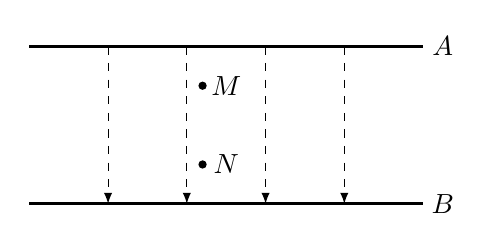
\begin{tikzpicture}[>=latex,scale=1.0]
  % \useasboundingbox(-1,-2)rectangle(8,6);
  \foreach \x in {0,2}
  {
      \draw[very thick] (0,\x) --(5,\x);
  }
  \node at (5.25,0){$B$};
  \node at (5.25,2){$A$};
  \foreach \x in {1, 2,3,4}
  {
      \draw[->, dashed](\x,2)--(\x,0);
  }   
  \node at (2.5,1.5){$M$};    \node at (2.5,.5){$N$};
  \fill (2.2,1.5) circle (1.5pt);\fill (2.2,.5) circle (1.5pt);
\end{tikzpicture}
\end{document}